\subsubsection{Adapters - Incoming}

\subsubsubsection{SchemaValidatorFactory} \label{SchemaValidatorFactory}
\begin{figure}[H]
    \centering
    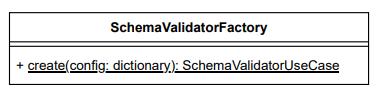
\includegraphics[width=0.65\textwidth]{assets/Backend/schema_validator_factory.png}
    \caption{Diagramma della classe SchemaValidatorFactory}
  \end{figure}
\begin{itemize}
    \item \textbf{Descrizione}: SchemaValidatorFactory si occupa della creazione di istanze di validatori di schema, come JsonSchemaValidatorAdapter, basandosi sulla configurazione fornita;
    \item \textbf{Metodi}:
    \begin{itemize}
        \item \texttt{+ \underline{create(config: dict)}}: restituisce un'istanza del validatore in base al valore associato alla chiave "validation\_file\_type".
    \end{itemize}
    \item \textbf{Dipendenze}:
    \begin{itemize}
        \item SchemaValidatorUseCase.
    \end{itemize}
\end{itemize}  

\subsubsubsection{JsonSchemaValidatorAdapter} \label{JsonSchemaValidatorAdapter}
\begin{figure}[H]
    \centering
    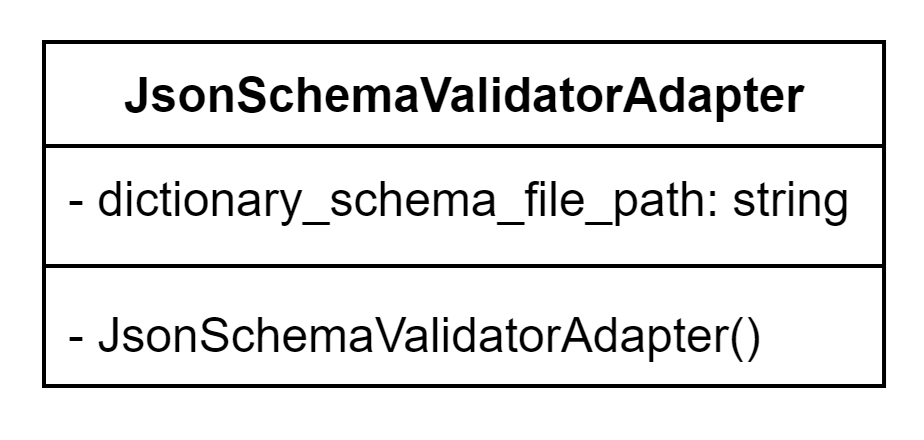
\includegraphics[width=0.55\textwidth]{assets/Backend/json_schema_validator_adapter.png}
    \caption{Diagramma della classe JsonSchemaValidatorAdapter}
  \end{figure}
\begin{itemize}
    \item \textbf{Descrizione}: JsonSchemaValidatorAdapter implementa il caso d'uso di validazione dello schema dei dizionari in formato \glossario{JSON};
    \item \textbf{Interfaccia implementata}: \hyperref[SchemaValidatorUseCase]{SchemaValidatorUseCase};
    \item \textbf{Attributi}:
    \begin{itemize}
        \item \texttt{dictionary\_schema\_file\_path}: percorso del file \glossario{JSON} che contiene lo schema dei dizionari dati.
    \end{itemize}
    \item \textbf{Metodi}:
    \begin{itemize}
        \item \texttt{JsonSchemaValidatorAdapter()}: costruttore della classe;
        \item \texttt{+ validate(dictionary\_content: string)}: valida il dizionario dati rispetto a uno schema predefinito.
    \end{itemize}
    \item \textbf{Dipendenze}:
    \begin{itemize}
        \item Utils.
    \end{itemize}
\end{itemize} 

\subsubsection{Outcoming - Adapters}

\subsubsubsection{DbManagerFactory} \label{DbManagerFactory}
\begin{figure}[H]
    \centering
    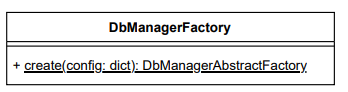
\includegraphics[width=0.65\textwidth]{assets/Backend/db_manager_factory.png}
    \caption{Diagramma della classe DbManagerFactory}
  \end{figure}
\begin{itemize}
    \item \textbf{Descrizione}: DbManagerFactory si occupa della creazione di istanze di gestori di \glossario{database} specifici, come SqlAlchemyDbManagerFactory, basandosi sulla configurazione fornita;
    \item \textbf{Metodi}:
    \begin{itemize}
        \item \texttt{+ \underline{create(config: dict)}}: restituisce un'istanza del gestore di database in base al valore associato alla chiave "db\_manager".
    \end{itemize}
    \item \textbf{Dipendenze}:
    \begin{itemize}
        \item DbManagerAbstractFactory.
    \end{itemize}
\end{itemize}

\subsubsubsection{SqlAlchemyDbManagerFactory} \label{SqlAlchemyDbManagerFactory}
\begin{figure}[H]
    \centering
    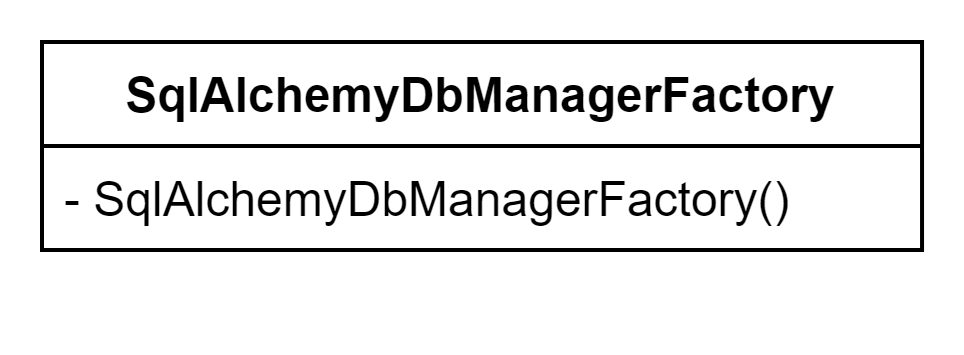
\includegraphics[width=0.55\textwidth]{assets/Backend/sql_alchemy_db_manager_factory.png}
    \caption{Diagramma della classe SqlAlchemyDbManagerFactory}
  \end{figure}
\begin{itemize}
    \item \textbf{Descrizione}: SqlAlchemyDbManagerFactory si occupa della creazione di istanze di classi per la gestione degli utenti e dei dizionari utilizzando \glossario{SQLAlchemy};
    \item \textbf{Interfaccia implementata}: \hyperref[DbManagerAbstractFactory]{DbManagerAbstractFactory};
    \item \textbf{Metodi}:
    \begin{itemize}
        \item \texttt{+ create\_authentication\_repository()}: restituisce un'istanza della classe SqlAlchemyAuthenticationRepositoryAdapter;
        \item \texttt{+ create\_dictionary\_repository()}: restituisce un'istanza della classe SqlAlchemyDictionaryRepositoryAdapter.
    \end{itemize}
    \item \textbf{Dipendenze}:
    \begin{itemize}
        \item AuthenticationRepository;
        \item DictionaryRepository.
    \end{itemize}
\end{itemize}

\subsubsubsection{SqlAlchemyAuthenticationRepositoryAdapter} \label{SqlAlchemyAuthenticationRepositoryAdapter}
\begin{figure}[H]
    \centering
    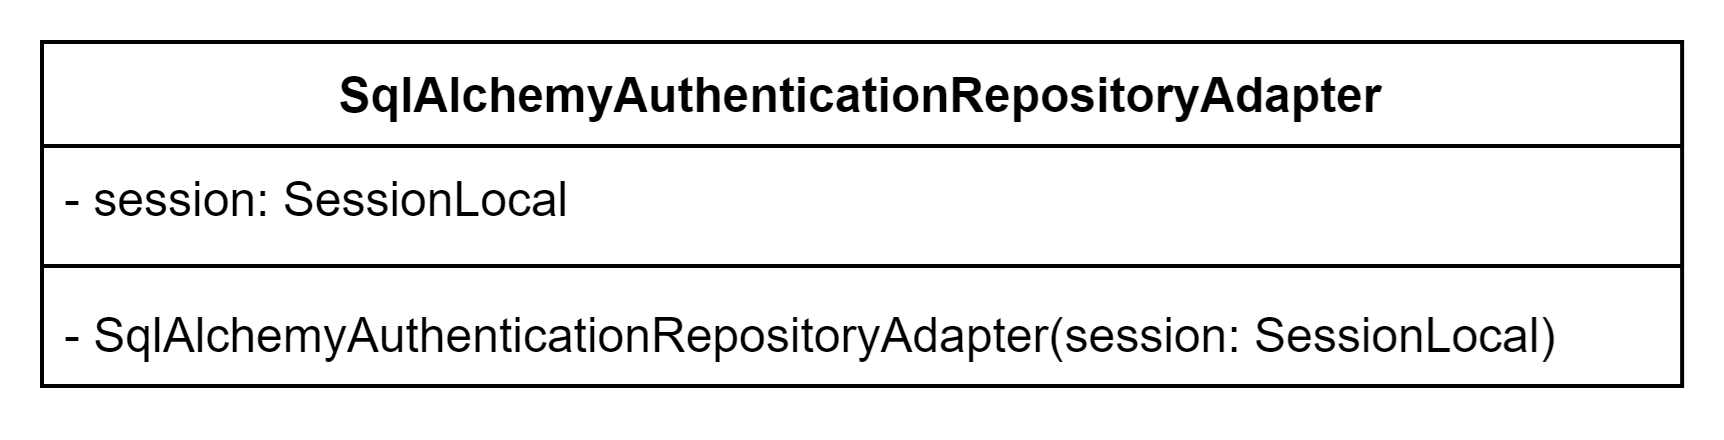
\includegraphics[width=0.75\textwidth]{assets/Backend/sql_alchemy_authentication_repository_adapter.png}
    \caption{Diagramma della classe SqlAlchemyAuthenticationRepositoryAdapter}
  \end{figure}
\begin{itemize}
    \item \textbf{Descrizione}: SqlAlchemyAuthenticationRepositoryAdapter interagisce con un database utilizzando \glossario{SQLAlchemy} per la gestione degli utenti;
    \item \textbf{Interfaccia implementata}: \hyperref[AuthenticationRepository]{AuthenticationRepository};
    \item \textbf{Attributi}:
    \begin{itemize}
        \item \texttt{session}: sessione di connessione al database.
    \end{itemize}
    \item \textbf{Metodi}:
    \begin{itemize}
        \item \texttt{SqlAlchemyAuthenticationRepositoryAdapter(session: SessionLocal)}: costruttore della classe;
        \item \texttt{+ get\_admin\_by\_username(username: string)}: recupera un admin dal database tramite il suo username.
    \end{itemize}
\end{itemize} 

\subsubsubsection{SqlAlchemyDictionaryRepositoryAdapter} \label{SqlAlchemyDictionaryRepositoryAdapter}
\begin{figure}[H]
    \centering
    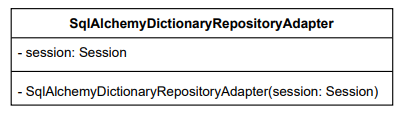
\includegraphics[width=0.65\textwidth]{assets/Backend/sql_alchemy_dictionary_repository_adapter.png}
    \caption{Diagramma della classe SqlAlchemyDictionaryRepositoryAdapter}
  \end{figure}
\begin{itemize}
    \item \textbf{Descrizione}: SqlAlchemyDictionaryRepositoryAdapter interagisce con un database utilizzando \glossario{SQLAlchemy} per la gestione dei dizionari;
    \item \textbf{Interfaccia implementata}: \hyperref[DictionaryRepository]{DictionaryRepository};
    \item \textbf{Attributi}:
    \begin{itemize}
        \item \texttt{session}: sessione di connessione al database.
    \end{itemize}
    \item \textbf{Metodi:}
    \begin{itemize}
        \item \texttt{SqlAlchemyDictionaryRepositoryAdapter(session: SessionLocal)}: costruttore della classe;
        \item \texttt{+ get\_all\_dictionaries()}: recupera tutti i dizionari dal database;
        \item \texttt{+ get\_dictionary\_by\_id(id: integer)}: recupera un dizionario tramite il suo ID;
        \item \texttt{+ get\_dictionary\_by\_name(name: string)}: recupera un dizionario tramite il suo nome;
        \item \texttt{+ create\_dictionary(name: string, description: string)}: crea un nuovo dizionario nel database;
        \item \texttt{+ update\_dictionary(id: integer, name: string, description: string)}: aggiorna i dati di un dizionario nel database;
        \item \texttt{+ delete\_dictionary(id: integer)}: elimina un dizionario dal database.
    \end{itemize}
\end{itemize} 

\subsubsubsection{EmbeddingsManagerFactory} \label{EmbeddingsManagerFactory}
\begin{figure}[H]
    \centering
    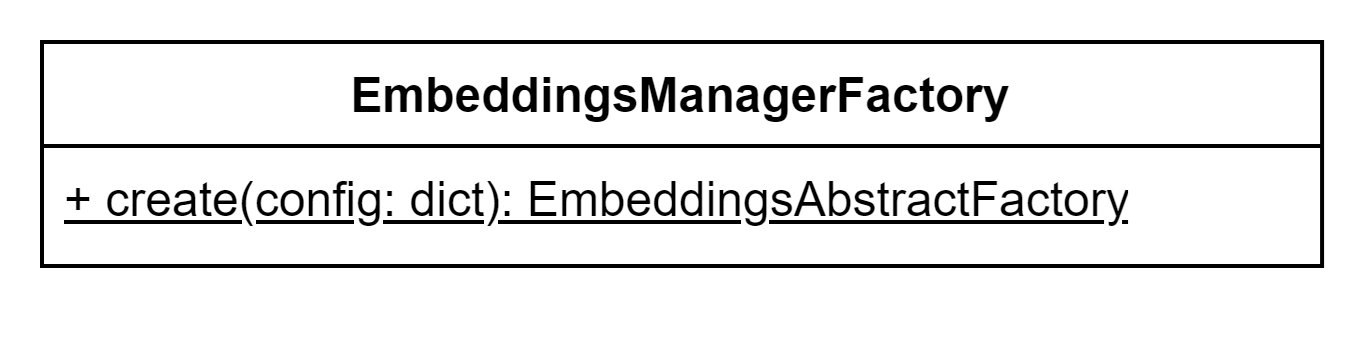
\includegraphics[width=0.65\textwidth]{assets/Backend/embeddings_manager_factory.png}
    \caption{Diagramma della classe EmbeddingsManagerFactory}
  \end{figure}
\begin{itemize}
    \item \textbf{Descrizione}: EmbeddingsManagerFactory si occupa della creazione di istanze di gestori di \glossario{embeddings}, come TxtaiEmbeddingsManagerFactory, basandosi sulla configurazione fornita;
    \item \textbf{Metodi}:
    \begin{itemize}
        \item \texttt{+ \underline{create(config: dict)}}: restituisce un'istanza del gestore di embeddings in base al valore associato alla chiave "embeddings\_type".
    \end{itemize}
    \item \textbf{Dipendenze}:
    \begin{itemize}
        \item EmbeddingsAbstractFactory.
    \end{itemize}
\end{itemize} 

\subsubsubsection{TxtaiEmbeddingsManagerFactory} \label{TxtaiEmbeddingsManagerFactory}
\begin{figure}[H]
    \centering
    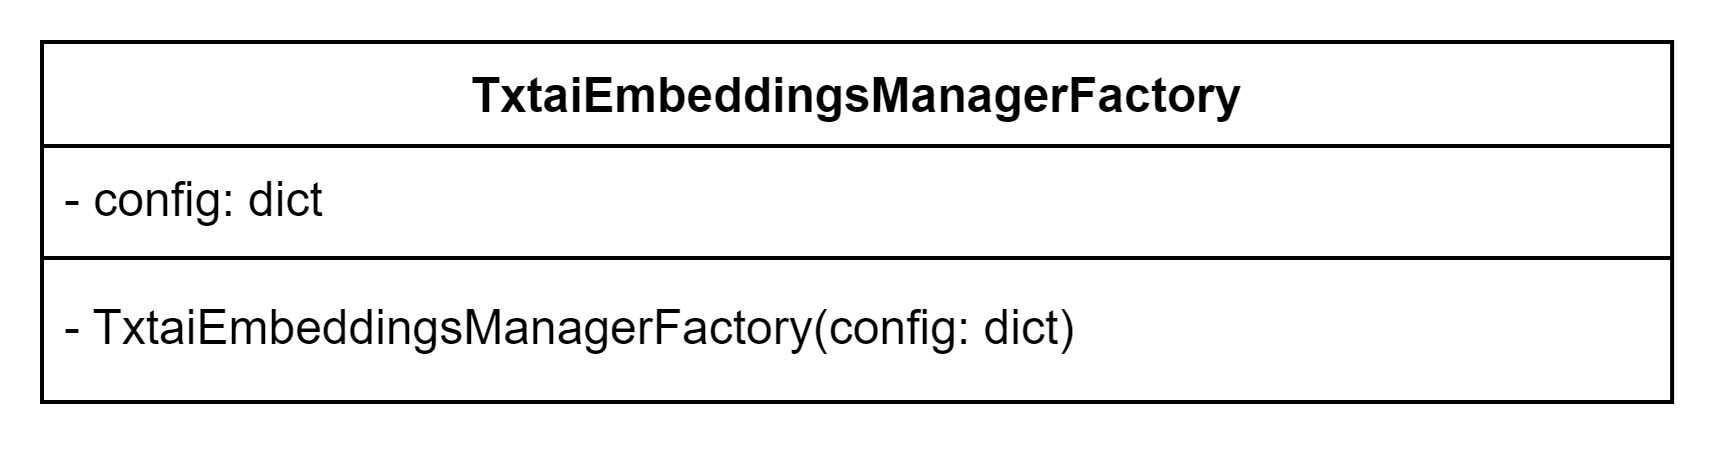
\includegraphics[width=0.7\textwidth]{assets/Backend/txtai_embeddings_manager_factory.png}
    \caption{Diagramma della classe TxtaiEmbeddingsManagerFactory}
  \end{figure}
\begin{itemize}
    \item \textbf{Descrizione}: TxtaiEmbeddingsManagerFactory si occupa della creazione di istanze di gestori degli \glossario{indici} e dei \glossario{prompt} utilizzando \glossario{txtai};
    \item \textbf{Interfaccia implementata}: \hyperref[EmbeddingsAbstractFactory]{EmbeddingsAbstractFactory};
    \item \textbf{Attributi}:
    \begin{itemize}
        \item \texttt{config}: dizionario di configurazione del sistema.
    \end{itemize}
    \item \textbf{Metodi}:
    \begin{itemize}
        \item \texttt{TxtaiEmbeddingsManagerFactory(config: dict)}: costruttore della classe;
        \item \texttt{create\_index\_manager(file\_repository: FileRepository)}: restituisce un'istanza della classe TxtaiIndexManagerAdapter, impostando parametri specifici per txtai;
        \item \texttt{create\_prompt\_manager\_with\_dependencies(index\_manager: IndexManagerPort, file\_repository: FileRepository)}: restituisce un'istanza della classe TxtaiPromptManagerAdapter;
        \item \texttt{create\_prompt\_manager(file\_repository: FileRepository)}: restituisce un'istanza della classe TxtaiPromptManagerAdapter, creata dopo aver generato un'istanza di TxtaiIndexManagerAdapter.
    \end{itemize}
    \item \textbf{Dipendenze}:
    \begin{itemize}
        \item FileRepository;
        \item IndexManagerPort;
        \item PromptManagerPort.
    \end{itemize}
\end{itemize} 

\subsubsubsection{TxtaiIndexManagerAdapter} \label{TxtaiIndexManagerAdapter}
\begin{figure}[H]
    \centering
    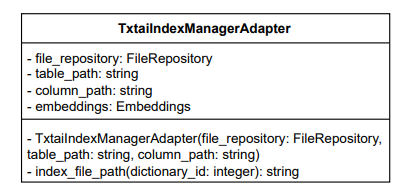
\includegraphics[width=0.6\textwidth]{assets/Backend/txtai_index_manager_adapter.png}
    \caption{Diagramma della classe TxtaiIndexManagerAdapter}
  \end{figure}
\begin{itemize}
    \item \textbf{Descrizione}: TxtaiIndexManagerAdapter gestisce le operazioni \glossario{CRUD} sugli indici utilizzando \glossario{txtai};
    \item \textbf{Interfaccia implementata}: \hyperref[IndexManagerPort]{IndexManagerPort};
    \item \textbf{Attributi}:
    \begin{itemize}
        \item \texttt{file\_repository}: istanza del gestore dei file;
        \item \texttt{indexes\_out\_file\_base\_path}: percorso della cartella contenente gli indici;
        \item \texttt{embeddings}: istanza di Embeddings utilizzata per la gestione degli embeddings.
    \end{itemize}
    \item \textbf{Metodi}:
    \begin{itemize}
        \item \texttt{TxtaiIndexManagerAdapter(file\_repository: FileRepository, table\_path:\\ string, column\_path: string)}: costruttore della classe;
        \item \texttt{+ get\_embeddings}: recupera l'istanza di Embeddings;
        \item \texttt{+ create\_or\_load\_index(dictionary\_id: integer)}: crea o ripristina l'indice per un dizionario;
        \item \texttt{+ create\_index(dictionary\_id: integer, save\_index: bool)}: crea un nuovo indice per un dizionario;
        \item \texttt{+ save\_index(dictionary\_id: integer)}: salva l'indice associato a un dizionario;
        \item \texttt{+ load\_index(dictionary\_id: integer)}: ripristina l'indice associato a un dizionario;
        \item \texttt{+ delete\_index(dictionary\_id: integer)}: elimina l'indice associato a un dizionario;
        \item \texttt{- index\_file\_path(dictionary\_id: integer)}: restituisce il percorso completo dell'indice associato a un dizionario.
    \end{itemize}
    \item \textbf{Dipendenze}:
    \begin{itemize}
        \item FileRepository.
    \end{itemize}
\end{itemize} 

\subsubsubsection{TxtaiPromptManagerAdapter} \label{TxtaiPromptManagerAdapter}
\begin{figure}[H]
    \centering
    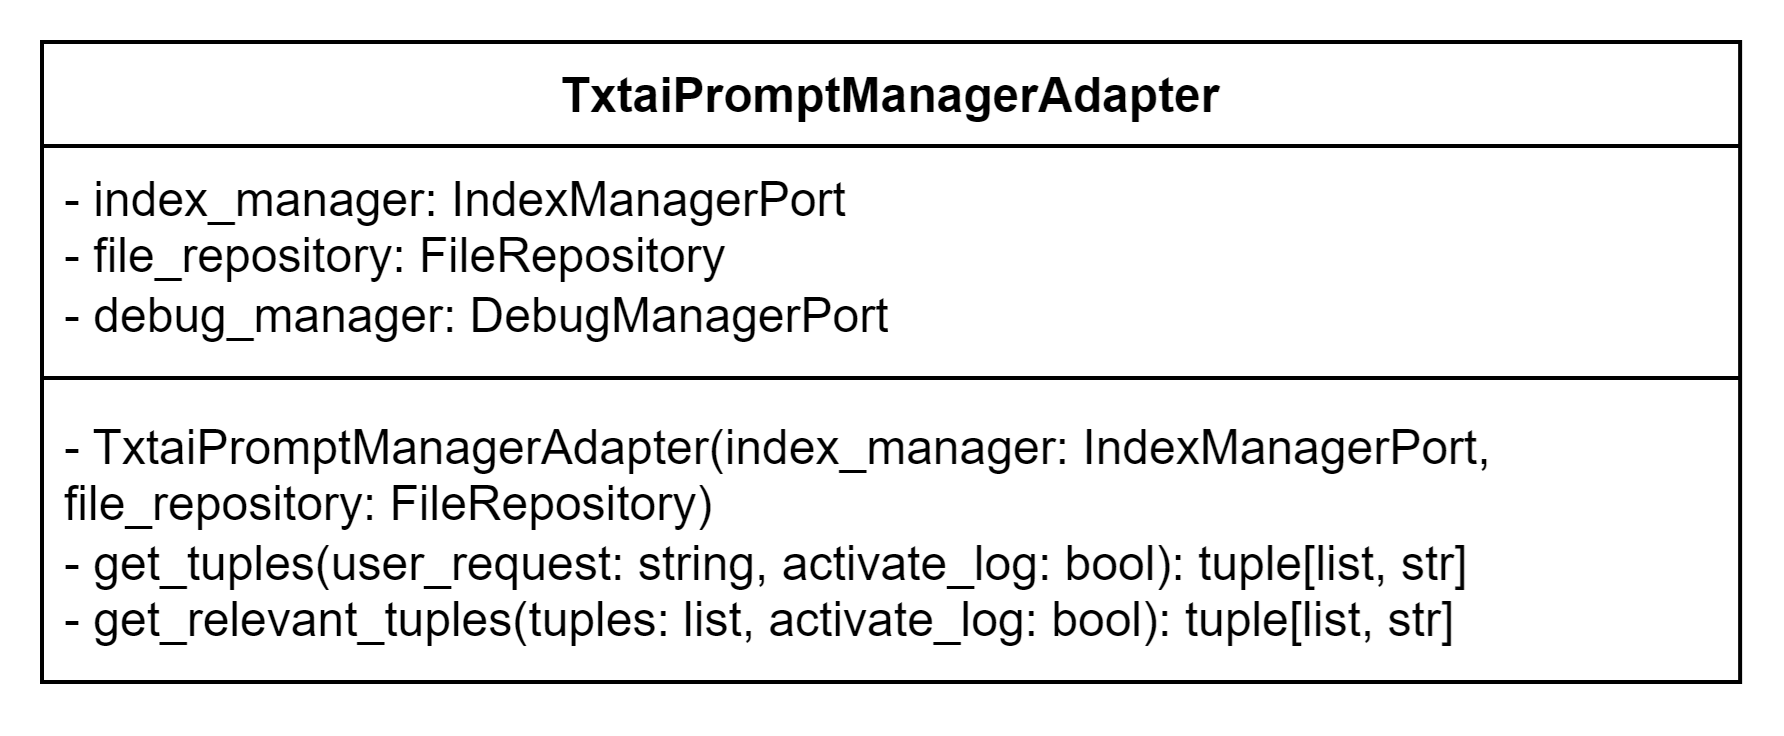
\includegraphics[width=0.75\textwidth]{assets/Backend/txtai_prompt_manager_adapter.png}
    \caption{Diagramma della classe TxtaiPromptManagerAdapter}
  \end{figure}
\begin{itemize}
    \item \textbf{Descrizione}: TxtaiPromptManagerAdapter gestisce la generazione di \glossario{prompt} utilizzando \glossario{txtai};
    \item \textbf{Interfaccia implementata}: \hyperref[PromptManagerPort]{PromptManagerPort};
    \item \textbf{Attributi}:
    \begin{itemize}
        \item \texttt{index\_manager}: istanza del gestore degli \glossario{indici};
        \item \texttt{file\_repository}: istanza del gestore dei file;
        \item \texttt{search\_algorithm}: istanza della classe utilizzata per gestire le operazioni di ricerca semantica.
    \end{itemize}
    \item \textbf{Metodi}:
    \begin{itemize}
        \item \texttt{TxtaiPromptManagerAdapter(index\_manager: IndexManagerPort, file\_repository:\\ FileRepository)}: costruttore della classe;
        \item \texttt{+ prompt\_generator(dictionary\_id: integer, user\_request: string, lang:\\ string, dbms: string, activate\_log: bool)}: carica l'indice associato a un dizionario e genera un prompt basato sulla richiesta dell'utente;
        \item \texttt{+ get\_index\_manager()}: restituisce l'istanza del gestore degli indici.
    \end{itemize}
    \item \textbf{Dipendenze}:
    \begin{itemize}
        \item IndexManagerPort;
        \item FileRepository;
        \item SearchAlgorithmPort.
    \end{itemize}
\end{itemize} 

\subsubsubsection{TxtaiSearchAlgorithmAdapter} \label{TxtaiSearchAlgorithmAdapter}
\begin{figure}[H]
    \centering
    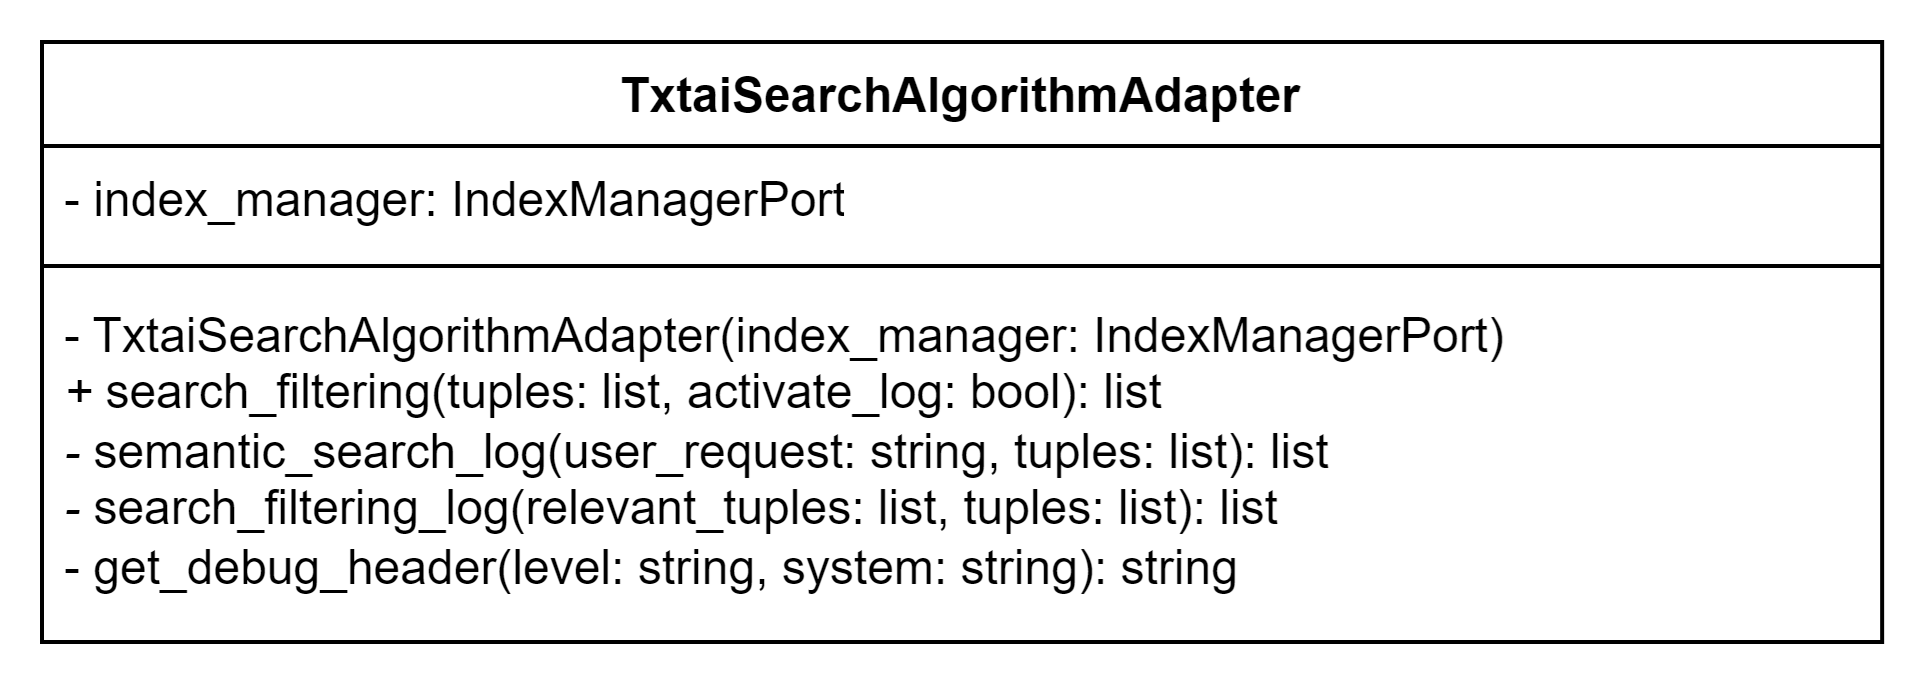
\includegraphics[width=0.75\textwidth]{assets/Backend/txtai_search_algorithm_adapter.png}
    \caption{Diagramma della classe TxtaiSearchAlgorithmAdapter}
  \end{figure}
\begin{itemize}
    \item \textbf{Descrizione}: TxtaiSearchAlgorithmAdapter fornisce funzionalità di ricerca semantica e di \glossario{logging} del processo di ricerca;
    \item \textbf{Interfaccia implementata}: \hyperref[SearchAlgorithmPort]{SearchAlgorithmPort};
    \item \textbf{Attributi}:
    \begin{itemize}
        \item \texttt{index\_manager}: istanza del gestore degli \glossario{indici}.
    \end{itemize}
    \item \textbf{Metodi}:
    \begin{itemize}
        \item \texttt{TxtaiSearchAlgorithmAdapter(index\_manager: IndexManagerPort)}: costruttore della classe;
        \item \texttt{+ semantic\_search(user\_request: string, activate\_log: bool)}: restituisce i risultati della ricerca semantica effettuata con txtai;
        \item \texttt{+ search\_filtering(tuples: list, activate\_log: bool)}: restituisce le tabelle considerate rilevanti dall'algoritmo di filtraggio implementato dal team;
        \item \texttt{- semantic\_search\_log(user\_request: string, tuples: list)}: restituisce il \glossario{log} della ricerca semantica effettuata con \glossario{txtai};
        \item \texttt{- search\_filtering\_log(relevant\_tuples: list, tuples: list)}: restituisce il log dell'algoritmo di filtraggio implementato dal team;
        \item \texttt{- get\_debug\_header(level: string, system: string)}: costruisce l'intestazione del log.
    \end{itemize}
    \item \textbf{Dipendenze}:
    \begin{itemize}
        \item IndexManagerPort.
    \end{itemize}
\end{itemize} 

\subsubsubsection{FileFactory} \label{FileFactory}
\begin{figure}[H]
    \centering
    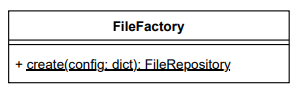
\includegraphics[width=0.6\textwidth]{assets/Backend/file_factory.png}
    \caption{Diagramma della classe FileFactory}
  \end{figure}
\begin{itemize}
    \item \textbf{Descrizione}: FileFactory si occupa della creazione di istanze di gestori di file, come JsonFileAdapter, basandosi sulla configurazione fornita;
    \item \textbf{Metodi}:
    \begin{itemize}
        \item \texttt{+ \underline{create(config: dict)}}: restituisce un'istanza del gestore di file in base al valore associato alla chiave "file\_type".
    \end{itemize}
    \item \textbf{Dipendenze}:
    \begin{itemize}
        \item FileRepository.
    \end{itemize}
\end{itemize} 

\subsubsubsection{JsonFileAdapter} \label{JsonFileAdapter}
\begin{figure}[H]
    \centering
    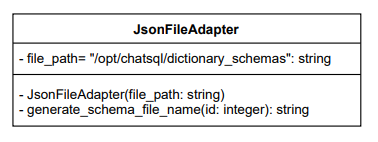
\includegraphics[width=0.6\textwidth]{assets/Backend/json_file_adapter.png}
    \caption{Diagramma della classe JsonFileAdapter}
  \end{figure}
\begin{itemize}
    \item \textbf{Descrizione}: JsonFileAdapter gestisce le operazioni \glossario{CRUD} sui file associati ai \glossario{dizionari dati};
    \item \textbf{Interfaccia implementata}: \hyperref[FileRepository]{FileRepository};
    \item \textbf{Attributi}:
    \begin{itemize}
        \item \texttt{file\_path}: percorso della cartella contenente i file dei dizionari dati;
    \end{itemize}
    \item \textbf{Metodi}:
    \begin{itemize}
        \item \texttt{JsonFileAdapter(file\_path: string)}: costruttore della classe;
        \item \texttt{+ save(id: integer, file: string)}: salva il file;
        \item \texttt{+ get\_file\_path(id: integer)}: restituisce il percorso del file;
        \item \texttt{+ delete(id: integer)}: elimina il file;
        \item \texttt{+ get\_preview(id: integer)}: recupera un'anteprima del file;
        \item \texttt{+ extract\_index\_metadata(id: integer)}: estrae i metadati per l'\glossario{indicizzazione};
        \item \texttt{+ extract\_schema\_metadata(id: integer, tuples: list)}: estrae i metadati in forma di \glossario{prompt};
        \item \texttt{- get\_json\_schema(id: integer)}: restituisce lo schema del file \glossario{JSON}.
    \end{itemize}
    \item \textbf{Dipendenze}:
    \begin{itemize}
        \item Utils.
    \end{itemize}
\end{itemize} 